\section{Introduction}
This project focuses on the game of Draughts, a strategic board game with profound combinatorial complexity. The Draughts, with its simple rules yet intricate strategic depth, offers an ideal testbed for AI algorithms. Our project aims to design and implement a set of diverse AI algorithms, each unique in its approach to decision-making and strategy formulation. These include the Random algorithm, offering baseline performance metrics; the Minimax Search algorithm, a classic approach in game AI emphasizing strategic depth; Reinforcement Learning, which seeks to optimize strategies through trial and error in a dynamic environment; and the Monte-Carlo Tree Search, a probabilistic model known for its effectiveness in dealing with the uncertainty and complexity inherent in Draughts.

\begin{figure}[t]
    \centering
    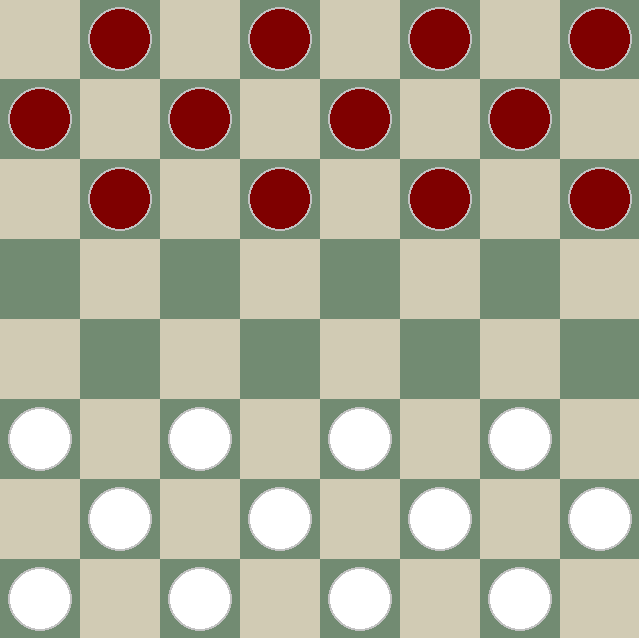
\includegraphics[width=\linewidth]{figures/board.png}
    \caption{Visulization of draught game board}
    \label{fig:board}
\end{figure}

% ------------------------------------
\subsection{State Space}

The board is shown in Figure \ref{fig:board}, there are a total of $8\times 8=64$ lattices on the board, but only $32$ of them are accessible for pieces. Each accessible lattice may be put on a black piece, a white piece, a white king, a black king, or nothing on it. So each accessible lattice may have $5$ status. So the total number of state spaces is $5^{32}\approx10^{22}$.

% ------------------------------------
\subsection{Motivation}
So far, we have learned various intelligence agents in courses, including search, adversarial search, bayesian network, Markov decision model, reinforcement learning, and machine learning. Draught, with simple rules but various states, is suitable for applying these methods to an intelligent agent. With this motivation, we implement random agents, minimax agents, MCTS agents, Q-Learning agents, and approximate Q-Learning agents. Also, we train a Neural Network to evaluate the final score for a state to improve the evaluation function. We compare the performance of each method against nondeterministic methods including random and MCTS and evaluate the strength of our evaluation function of the game state. 

% \textcolor{red}{motivation?}
